% =====================================================================
%  QuestCash — Entregable ED, Semana 1
%  Separacion publico/privado, hashing y cifrado en reposo
%  Compilar con:  pdflatex reporte_semanaED1.tex   (dos veces)
%
%  Continuación directa del reporte de la semana 2 (autenticación JWT):
%  reutiliza su preámbulo, paleta y estilos.
% =====================================================================
\documentclass[11pt,letterpaper]{article}

\usepackage[utf8]{inputenc}
\usepackage[T1]{fontenc}
\usepackage[margin=2.4cm,top=2.8cm,bottom=2.6cm]{geometry}
\usepackage{xcolor}
\usepackage{graphicx}
\usepackage{booktabs}
\usepackage{longtable}
\usepackage{array}
\usepackage{enumitem}
\usepackage{fancyhdr}
\usepackage{titlesec}
\usepackage{caption}
\usepackage{tcolorbox}
\usepackage{listings}
\usepackage{tikz}
\usepackage{amsmath}
\usepackage{amssymb}
\usepackage[hidelinks]{hyperref}

\usetikzlibrary{positioning,arrows.meta,shapes.geometric,calc,fit,backgrounds}
\tcbuselibrary{skins,breakable}

% ---------- Español (sin babel: se renombran los rótulos a mano) ----------
\renewcommand{\tablename}{Tabla}
\renewcommand{\figurename}{Figura}
\renewcommand{\refname}{Referencias}
\renewcommand{\contentsname}{Contenido}

% ---------- Paleta (idéntica a la del reporte de la semana 2) ----------
\definecolor{qcNavy}{HTML}{0F2E4C}
\definecolor{qcBlue}{HTML}{2563EB}
\definecolor{qcGreen}{HTML}{16A34A}
\definecolor{qcRed}{HTML}{DC2626}
\definecolor{qcAmber}{HTML}{B45309}
\definecolor{qcGray}{HTML}{6B7280}
\definecolor{qcLight}{HTML}{F3F4F6}
\definecolor{qcCodeBg}{HTML}{111827}

% ---------- Encabezado / pie ----------
\pagestyle{fancy}
\fancyhf{}
\fancyhead[L]{\footnotesize\color{qcGray}QuestCash · Entregable ED — Semana 1}
\fancyhead[R]{\footnotesize\color{qcGray}Separación de planos · hashing · cifrado}
\fancyfoot[C]{\footnotesize\color{qcGray}\thepage}
\renewcommand{\headrulewidth}{0.4pt}
\renewcommand{\headrule}{\hbox to\headwidth{\color{qcLight}\leaders\hrule height \headrulewidth\hfill}}

% ---------- Títulos ----------
\titleformat{\section}{\Large\bfseries\color{qcNavy}}{\thesection.}{0.6em}{}
\titleformat{\subsection}{\large\bfseries\color{qcNavy}}{\thesubsection}{0.6em}{}
\titlespacing*{\section}{0pt}{1.6em}{0.7em}

\captionsetup{font=small,labelfont={bf,color=qcNavy}}

% ---------- Estilos de código ----------
\lstdefinestyle{terminal}{
  extendedchars=true,
  inputencoding=utf8,
  basicstyle=\ttfamily\fontsize{6}{7.2}\selectfont\color{white},
  backgroundcolor=\color{qcCodeBg},
  breaklines=true, columns=fullflexible, keepspaces=true,
  showstringspaces=false, frame=none, xleftmargin=6pt, xrightmargin=4pt,
  literate={á}{{\'a}}1 {é}{{\'e}}1 {í}{{\'i}}1 {ó}{{\'o}}1 {ú}{{\'u}}1
           {ñ}{{\~n}}1 {Á}{{\'A}}1 {É}{{\'E}}1 {Í}{{\'I}}1 {Ó}{{\'O}}1 {Ú}{{\'U}}1
           {¿}{{?}}1 {¡}{{!}}1 {—}{{---}}3 {–}{{--}}2 {º}{{\textdegree}}1
           {“}{{"}}1 {”}{{"}}1 {‘}{{'}}1 {’}{{'}}1
}

\lstdefinestyle{conf}{
  extendedchars=true,
  inputencoding=utf8,
  basicstyle=\ttfamily\scriptsize,
  keywordstyle=\color{qcBlue}\bfseries,
  commentstyle=\color{qcGreen}\itshape,
  stringstyle=\color{qcAmber},
  numbers=left, numberstyle=\tiny\color{qcGray}, numbersep=8pt,
  breaklines=true, columns=fullflexible, keepspaces=true,
  showstringspaces=false, frame=leftline, framesep=6pt,
  rulecolor=\color{qcLight}, xleftmargin=16pt,
  morecomment=[l]{\#},
  literate={á}{{\'a}}1 {é}{{\'e}}1 {í}{{\'i}}1 {ó}{{\'o}}1 {ú}{{\'u}}1
           {ñ}{{\~n}}1 {Á}{{\'A}}1 {É}{{\'E}}1 {Í}{{\'I}}1 {Ó}{{\'O}}1 {Ú}{{\'U}}1
           {—}{{---}}3 {–}{{--}}2 {«}{{<<}}2 {»}{{>>}}2 {¿}{{?}}1 {º}{{\textdegree}}1
}

\lstdefinelanguage{nginxconf}{
  morekeywords={http,server,upstream,location,events,listen,proxy_pass,
    proxy_set_header,proxy_next_upstream,proxy_next_upstream_tries,
    add_header,access_log,error_log,log_format,include,worker_processes,
    worker_connections,keepalive,max_fails,fail_timeout,stub_status,
    return,allow,deny,server_name,server_tokens,sendfile,tcp_nopush,
    proxy_http_version,proxy_connect_timeout,proxy_send_timeout,proxy_read_timeout},
  morecomment=[l]{\#},
  morestring=[b]",
  sensitive=true,
}

\lstdefinelanguage{yamlqc}{
  morekeywords={services,image,container_name,restart,environment,volumes,
    ports,depends_on,networks,build,context,dockerfile,command,healthcheck,
    condition,cap_add,security_opt,driver,hostname,name},
  morecomment=[l]{\#},
  morestring=[b]",
  sensitive=true,
}

% ---------- Cajas ----------
\newtcolorbox{consola}[1][]{
  enhanced, breakable,
  colback=qcCodeBg, colframe=qcNavy, boxrule=0.6pt, arc=2pt,
  left=2pt, right=2pt, top=4pt, bottom=4pt,
  fonttitle=\ttfamily\scriptsize\bfseries, coltitle=white, colbacktitle=qcNavy,
  #1
}

\newtcolorbox{nota}[1][]{
  enhanced, breakable,
  colback=qcLight, colframe=qcGray, boxrule=0.4pt, arc=2pt,
  left=8pt, right=8pt, top=6pt, bottom=6pt,
  #1
}

\newtcolorbox{alerta}[1][]{
  enhanced, breakable,
  colback=qcAmber!8, colframe=qcAmber, boxrule=0.8pt, arc=2pt,
  left=8pt, right=8pt, top=6pt, bottom=6pt,
  #1
}

% ---------- Recuadro de captura pendiente ----------
% Marca de forma inequívoca dónde va cada evidencia visual. No se
% incluyen imágenes simuladas: o es una captura real, o es un hueco.
\newtcolorbox{captura}[2]{
  enhanced, breakable,
  colback=white, colframe=qcGray, boxrule=0.8pt, arc=3pt,
  borderline={0.8pt}{0pt}{qcGray,dashed},
  left=10pt, right=10pt, top=8pt, bottom=8pt,
  title={\ttfamily\scriptsize\bfseries CAPTURA #1},
  fonttitle=\ttfamily\scriptsize\bfseries, coltitle=white, colbacktitle=qcGray,
  after title={\hfill\normalfont\itshape\scriptsize #2}
}

% ---------- Marcadores ----------
\newcommand{\ok}{\textcolor{qcGreen}{\textbf{\checkmark}}}
\newcommand{\pend}{\textcolor{qcAmber}{\textbf{pendiente}}}
\newcommand{\http}[2]{\textcolor{#1}{\texttt{\textbf{#2}}}}


\lstdefinestyle{py}{
  extendedchars=true,
  inputencoding=utf8,
  language=Python,
  basicstyle=\ttfamily\scriptsize,
  keywordstyle=\color{qcBlue}\bfseries,
  commentstyle=\color{qcGreen}\itshape,
  stringstyle=\color{qcAmber},
  numbers=left, numberstyle=\tiny\color{qcGray}, numbersep=8pt,
  breaklines=true, columns=fullflexible, keepspaces=true,
  showstringspaces=false, frame=leftline, framesep=6pt,
  rulecolor=\color{qcLight}, xleftmargin=16pt,
  literate={á}{{\'a}}1 {é}{{\'e}}1 {í}{{\'i}}1 {ó}{{\'o}}1 {ú}{{\'u}}1
           {ñ}{{\~n}}1 {Á}{{\'A}}1 {É}{{\'E}}1 {Í}{{\'I}}1 {Ó}{{\'O}}1 {Ú}{{\'U}}1
           {—}{{---}}3 {–}{{--}}2 {¿}{{?}}1 {¡}{{!}}1 {º}{{\textdegree}}1
           {“}{{"}}1 {”}{{"}}1 {’}{{'}}1
}

\lstdefinestyle{sql}{
  extendedchars=true, inputencoding=utf8,
  basicstyle=\ttfamily\scriptsize,
  keywordstyle=\color{qcBlue}\bfseries,
  morekeywords={SELECT,FROM,WHERE,UPDATE,SET,ALTER,TABLE,ADD,COLUMN,CREATE,UNIQUE,INDEX,ON,IN,AND,OR,NOT,NULL},
  breaklines=true, columns=fullflexible, keepspaces=true,
  showstringspaces=false, frame=leftline, framesep=6pt,
  rulecolor=\color{qcLight}, xleftmargin=16pt,
}

\newtcolorbox{bien}[1][]{
  enhanced, breakable,
  colback=qcGreen!7, colframe=qcGreen, boxrule=0.8pt, arc=2pt,
  left=8pt, right=8pt, top=6pt, bottom=6pt,
  #1
}
\begin{document}

% =====================  PORTADA  =====================
\begin{titlepage}
\centering
\vspace*{2.2cm}

{\color{qcBlue}\rule{\textwidth}{2.5pt}}

\vspace{0.9cm}
{\Huge\bfseries\color{qcNavy} QuestCash\par}
\vspace{0.4cm}
{\LARGE\color{qcNavy} Separación de planos, hashing de contraseñas\\ y cifrado en reposo\par}

\vspace{0.5cm}
{\color{qcBlue}\rule{\textwidth}{2.5pt}}

\vspace{1.4cm}
{\large\bfseries Entregable ED — Semana 1\par}
\vspace{0.5cm}
{\large\itshape Que lo público sea solo la puerta, y que lo que está\\ guardado no se pueda leer\par}

\vspace{2.0cm}

\begin{tabular}{@{}>{\bfseries\color{qcNavy}}l l@{}}
\toprule
Proyecto integrador & QuestCash \\
Materia             & Seguridad Informática \\
Equipo              & Proyecto QuestCash \\
Componentes         & \texttt{questcash\_web} (Flask) · \texttt{questcash\_mobile} (Expo) \\
Infraestructura     & Docker Compose · Nginx · PostgreSQL / SQLite \\
Producción          & Render (plan free), dominio \texttt{.onrender.com} \\
Autor               & Armando Yael Contreras Bejarano \\
Fecha               & 17 de agosto de 2026 \\
\bottomrule
\end{tabular}

\vfill
\begin{nota}
\small
\textbf{Sobre las evidencias de este documento.} Todo el código que aparece
aquí son \textbf{archivos reales del proyecto} —\texttt{crypto\_utils.py},
\texttt{password\_hashing.py}, \texttt{models.py},
\texttt{docker-compose.segmentado.yml}— y las salidas de consola se obtuvieron
\textbf{ejecutando} los scripts de \texttt{docs/semanaED1/} contra la base de
datos del proyecto. No hay salidas escritas a mano.

Las evidencias que exigen levantar Docker o Postman aparecen como
\textbf{recuadros marcados}, no como imágenes simuladas: cada recuadro indica
exactamente qué debe mostrar y qué comando lo produce.
\end{nota}
\end{titlepage}

\tableofcontents
\newpage

% =====================  1. INTRODUCCIÓN  =====================
\section{Introducción y alcance}

Esta entrega cierra cuatro puntos sobre el proyecto integrador QuestCash, una
aplicación de ahorro por metas con \emph{backend} Flask y aplicación móvil en
Expo:

\begin{enumerate}[leftmargin=1.6em,itemsep=3pt]
  \item Determinar qué parte del sistema es \textbf{pública} y cuál es
        \textbf{privada}.
  \item \textbf{Separar} ambas partes en instancias distintas, de modo que la
        privada no sea alcanzable desde Internet.
  \item Garantizar que las contraseñas se guardan \textbf{hasheadas} con una
        función lenta y salada, nunca en claro ni con MD5 o SHA-1.
  \item Identificar qué \textbf{otros datos} necesitan cifrado en reposo e
        implementarlo.
\end{enumerate}

Los puntos 1 y 2 ya estaban parcialmente resueltos desde la semana 3: la
aplicación corre detrás de Nginx y PostgreSQL nunca ha publicado un puerto.
Esta entrega los formaliza, los hace explícitos en un archivo de composición
dedicado y —lo importante— añade una prueba que los verifica en vez de
declararlos.

El punto 3 estaba resuelto desde el inicio del proyecto, pero la revisión
detectó que la política de hashing estaba repartida entre dos archivos y usaba
los parámetros por omisión de la biblioteca. Se centralizó y se endureció.

El punto 4 es trabajo nuevo: hasta esta semana, los datos personales de los
usuarios estaban guardados en texto plano.

\begin{alerta}
\textbf{Hallazgo que motivó la mitad de este trabajo.} Antes de esta entrega,
cualquiera que obtuviera una copia del archivo \texttt{questcash.db} o del
volumen de PostgreSQL podía leer los nombres, los correos y las notas de
gastos de las 25 cuentas registradas con un simple \texttt{SELECT}. La
contraseña estaba protegida; todo lo demás, no. El
\hyperref[sec:cifrado]{apartado 5} corrige eso.
\end{alerta}

% =====================  2. CLASIFICACIÓN  =====================
\section{Qué es público y qué es privado}

\subsection{El criterio}

La frontera no se traza por «qué es importante» sino por una pregunta
operativa: \textbf{¿este componente necesita que un desconocido de Internet
pueda abrirle una conexión?}

Si la respuesta es sí, es público y hay que asumir que estará bajo ataque
permanente. Si es no, es privado, y entonces exponerlo no aporta nada y solo
agrega superficie de ataque. Con ese criterio, la aplicación web es pública
—alguien tiene que poder registrarse— y la base de datos es privada, porque
ningún cliente legítimo habla con PostgreSQL directamente: hablan con la
aplicación, y es la aplicación quien decide qué puede ver cada usuario.

\subsection{Inventario de componentes}

\begin{center}
\small
\begin{tabular}{@{}>{\raggedright\arraybackslash}p{4.3cm} c >{\raggedright\arraybackslash}p{7.4cm}@{}}
\toprule
\textbf{Componente} & \textbf{Plano} & \textbf{Por qué} \\
\midrule
App móvil Expo (\texttt{questcash\_mobile})
  & Público
  & Se instala en el teléfono del usuario. Todo lo que lleva dentro debe
    considerarse conocido por un atacante: no guarda secretos, solo el JWT en
    \texttt{expo-secure-store}. \\[3pt]
Vistas HTML de Flask (\texttt{/login}, \texttt{/dashboard}, …)
  & Público
  & Es la interfaz web del producto. \\[3pt]
API REST \texttt{/api/v1}
  & Público
  & Es la puerta que consume la app móvil. Actúa como \emph{API gateway}:
    autentica con JWT y es el único camino hacia los datos. \\[3pt]
Archivos estáticos (\texttt{/static})
  & Público
  & CSS, imágenes e insignias. \\[3pt]
\midrule
Lógica de negocio (\texttt{app.py}, \texttt{api.py}, \texttt{ia/})
  & Frontera
  & Se ejecuta dentro del proceso público, pero su código y sus reglas de
    autorización no se exponen. Es la única pieza que pertenece a los dos
    planos. \\[3pt]
\midrule
PostgreSQL / SQLite
  & \textbf{Privado}
  & Ningún cliente legítimo se conecta a la base. Publicar el 5432 solo
    habilitaría ataques de fuerza bruta contra las credenciales de la base. \\[3pt]
Volumen de datos (\texttt{qc\_pgdata}) y respaldos
  & \textbf{Privado}
  & Contienen el estado completo del sistema. Un respaldo filtrado es una
    fuga total. \\[3pt]
Claves y secretos (\texttt{SECRET\_KEY}, \texttt{JWT\_SECRET\_KEY}, \texttt{DATA\_ENC\_KEY}, \texttt{BLIND\_INDEX\_KEY})
  & \textbf{Privado}
  & Viven en variables de entorno. \texttt{.env} está en \texttt{.gitignore};
    en Render, en el panel de \emph{Environment}. \\[3pt]
Panel de monitoreo (Netdata \texttt{:19999})
  & \textbf{Privado}
  & Revela la topología interna y el estado de los contenedores. Solo se abre
    en la red local del laboratorio. \\[3pt]
Datasets ENIGH (\texttt{data/raw}, \textasciitilde 750\,MB)
  & \textbf{Privado}
  & No se sirven ni se copian a la imagen: están excluidos en
    \texttt{.dockerignore}. \\
\bottomrule
\end{tabular}
\captionof{table}{Clasificación de cada componente de QuestCash.}
\end{center}

\subsection{Inventario de datos}
\label{sec:inventario-datos}

La misma pregunta, aplicada ahora a los datos, decide qué protección le toca a
cada campo. Hay tres respuestas posibles y no son intercambiables:

\begin{center}
\small
\begin{tabular}{@{}>{\raggedright\arraybackslash}p{3.9cm} >{\raggedright\arraybackslash}p{3.8cm} >{\raggedright\arraybackslash}p{7.0cm}@{}}
\toprule
\textbf{¿La app necesita\ldots} & \textbf{Mecanismo} & \textbf{Por qué} \\
\midrule
\ldots solo \emph{comprobar} el valor?
  & \textbf{Hash} (scrypt)
  & Irreversible a propósito. Ni el administrador de la base puede recuperar
    el dato original. \\[3pt]
\ldots \emph{leer} el valor de vuelta?
  & \textbf{Cifrado} (AES-256-GCM)
  & Reversible con la clave, ilegible sin ella. \\[3pt]
\ldots \emph{buscar} por el valor exacto?
  & \textbf{Índice ciego} (HMAC-SHA256)
  & Determinista para poder consultar, con clave para que no se pueda atacar
    por diccionario. \\
\bottomrule
\end{tabular}
\captionof{table}{Los tres mecanismos y cuándo aplica cada uno.}
\end{center}

\vspace{0.4em}

\begin{center}
\small
\begin{tabular}{@{}>{\raggedright\arraybackslash}p{4.6cm} >{\raggedright\arraybackslash}p{2.4cm} >{\raggedright\arraybackslash}p{4.6cm} c@{}}
\toprule
\textbf{Dato} & \textbf{Sensibilidad} & \textbf{Protección} & \textbf{Estado} \\
\midrule
\texttt{usuarios.password\_hash} & Credencial   & scrypt (\texttt{32768:8:3}) + sal   & \ok \\
\texttt{usuarios.correo}         & PII / identificador & AES-256-GCM + índice ciego  & \ok \\
\texttt{usuarios.nombre}         & PII          & AES-256-GCM                        & \ok \\
\texttt{usuarios.alias}          & PII          & AES-256-GCM                        & \ok \\
\texttt{movimientos.nota}        & Detalle financiero & AES-256-GCM                  & \ok \\
\texttt{gastos.descripcion}      & Detalle financiero & AES-256-GCM                  & \ok \\
Token JWT                        & Credencial   & Firmado HS256; en el cliente, \texttt{expo-secure-store} (Keychain / Keystore) & \ok \\
\texttt{DATA\_ENC\_KEY}, \texttt{BLIND\_INDEX\_KEY} & Clave maestra & Variable de entorno, fuera del repositorio & \ok \\
\midrule
\texttt{gastos.monto}, \texttt{quests.monto\_objetivo} & Financiero & Sin cifrar (ver nota) & --- \\
\texttt{usuarios.foto\_perfil}   & PII          & Nombre de archivo en claro; el archivo vive en \texttt{/static/uploads} & \pend \\
\bottomrule
\end{tabular}
\captionof{table}{Qué se protege, cómo, y qué queda pendiente.}
\end{center}

\begin{nota}
\textbf{Por qué los montos no se cifran.} La aplicación calcula sobre ellos:
suma aportes, compara contra la meta, agrupa gastos por categoría y saca
estadísticas. Un campo cifrado no se puede sumar ni comparar en SQL, así que
cifrarlos obligaría a traer todas las filas a memoria y operar en Python
—lo que rompe el rendimiento y, sobre todo, no protege gran cosa: un monto
suelto sin nombre ni concepto asociados dice muy poco. Lo que sí identifica a
una persona —quién es y en qué gastó— es justamente lo que sí quedó cifrado.
La alternativa real para esto es cifrado a nivel de volumen o \emph{Transparent
Data Encryption}, que se discute en \S\ref{sec:capas}.
\end{nota}

% =====================  3. SEPARACIÓN  =====================
\section{Separación del plano público y el privado}

\subsection{Arquitectura}

\begin{figure}[h!]
\centering
\resizebox{\textwidth}{!}{%
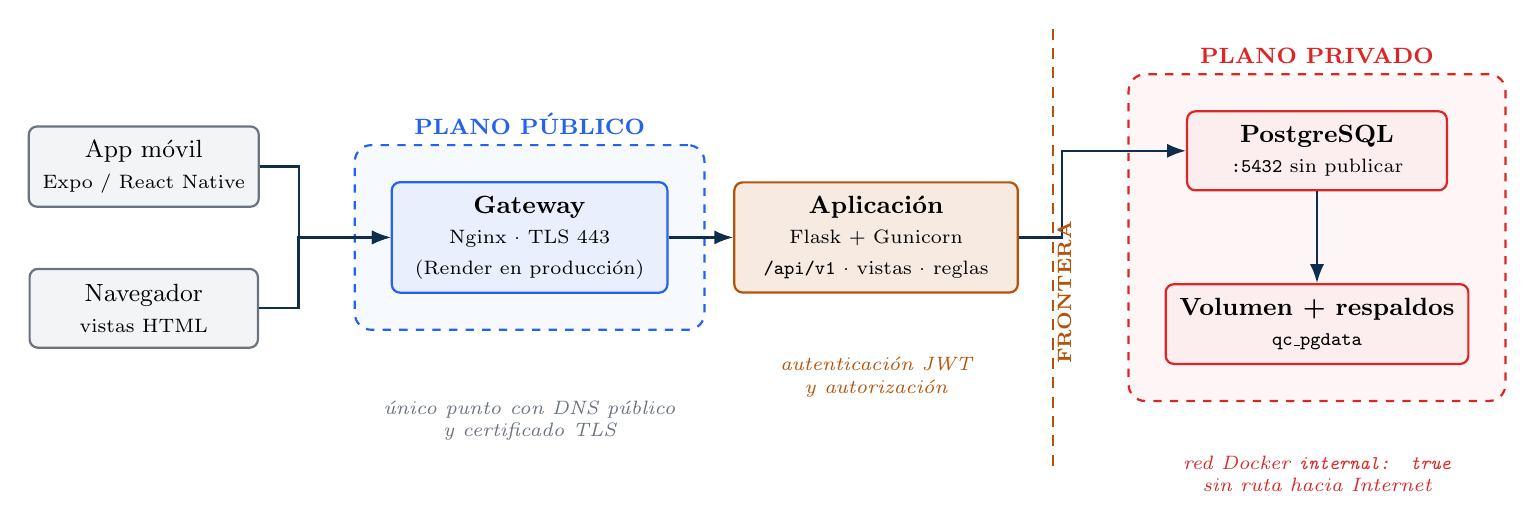
\begin{tikzpicture}[
  font=\small,
  caja/.style={rounded corners=3pt, draw, thick, align=center, minimum height=1.0cm, inner sep=5pt},
  pub/.style ={caja, fill=qcBlue!10,  draw=qcBlue},
  fron/.style={caja, fill=qcAmber!12, draw=qcAmber, thick},
  priv/.style={caja, fill=qcRed!8,    draw=qcRed},
  cli/.style ={caja, fill=qcLight,    draw=qcGray},
  flecha/.style={-{Latex[length=2.4mm]}, thick, draw=qcNavy},
]

% ---- Clientes ----
\node[cli, minimum width=2.9cm] (movil)  at (0,1.1) {App móvil\\\scriptsize Expo / React Native};
\node[cli, minimum width=2.9cm] (nav)    at (0,-0.7) {Navegador\\\scriptsize vistas HTML};

% ---- Plano público ----
\node[pub, minimum width=3.5cm] (gw) at (4.9,0.2)
     {\textbf{Gateway}\\\scriptsize Nginx · TLS 443\\\scriptsize (Render en producción)};

% ---- Frontera ----
\node[fron, minimum width=3.6cm] (app) at (9.3,0.2)
     {\textbf{Aplicación}\\\scriptsize Flask + Gunicorn\\\scriptsize \texttt{/api/v1} · vistas · reglas};

% ---- Plano privado ----
\node[priv, minimum width=3.3cm] (db)  at (14.9,1.3)
     {\textbf{PostgreSQL}\\\scriptsize \texttt{:5432} sin publicar};
\node[priv, minimum width=3.3cm] (vol) at (14.9,-0.9)
     {\textbf{Volumen + respaldos}\\\scriptsize \texttt{qc\_pgdata}};

% ---- Flechas ----
\draw[flecha] (movil.east) -- ++(0.5,0) |- (gw.west);
\draw[flecha] (nav.east)   -- ++(0.5,0) |- (gw.west);
\draw[flecha] (gw)  -- (app);
\draw[flecha] (app.east) -- ++(0.55,0) |- (db.west);
\draw[flecha] (db)  -- (vol);

% ---- Zonas ----
\begin{scope}[on background layer]
\node[draw=qcBlue, dashed, thick, rounded corners=6pt, fill=qcBlue!4,
      fit=(gw), inner sep=13pt, label={[qcBlue,font=\bfseries\footnotesize]above:PLANO PÚBLICO}] (zpub) {};
\node[draw=qcRed, dashed, thick, rounded corners=6pt, fill=qcRed!4,
      fit=(db)(vol), inner sep=13pt, label={[qcRed,font=\bfseries\footnotesize]above:PLANO PRIVADO}] (zpriv) {};
\end{scope}

% ---- Línea de frontera ----
\draw[qcAmber, thick, dash pattern=on 4pt off 3pt] (11.55,-2.7) -- (11.55,2.85);
\node[qcAmber, font=\bfseries\scriptsize, rotate=90, anchor=south] at (11.9,-0.5) {FRONTERA};

% ---- Etiquetas ----
\node[font=\scriptsize\itshape, qcGray, anchor=north, align=center] at (4.9,-1.75)
     {único punto con DNS público\\y certificado TLS};
\node[font=\scriptsize\itshape, qcRed, anchor=north, align=center] at (14.9,-2.45)
     {red Docker \texttt{internal: true}\\sin ruta hacia Internet};
\node[font=\scriptsize\itshape, qcAmber, anchor=north, align=center] at (9.3,-1.2)
     {autenticación JWT\\y autorización};

\end{tikzpicture}}
\caption{Arquitectura de QuestCash con la frontera explícita. La aplicación es
el único componente que pertenece a los dos planos, y por tanto el único camino
posible desde Internet hasta los datos.}
\end{figure}

\subsection{Cómo se implementa la separación}

Un diagrama no separa nada. La separación real está en
\texttt{docker-compose.segmentado.yml} (Anexo C) y se sostiene en tres
decisiones concretas:

\begin{enumerate}[leftmargin=1.6em,itemsep=5pt]
  \item \textbf{Un solo servicio publica puertos.} Solo \texttt{gateway} tiene
        sección \texttt{ports:}. Ni la aplicación ni PostgreSQL son alcanzables
        desde la máquina anfitriona, y por lo tanto tampoco desde Internet. En
        Docker, \emph{no publicar un puerto} es la forma más fuerte de cerrarlo:
        no hay regla de firewall que anular porque no hay nada escuchando en la
        interfaz del anfitrión.

  \item \textbf{Dos redes que no se tocan.} \texttt{gateway} vive únicamente en
        la red \texttt{publica}; \texttt{db} vive únicamente en la red
        \texttt{privada}. No comparten segmento. Si alguien comprometiera el
        Nginx, no tendría siquiera resolución DNS hacia \texttt{db}: tendría
        que atravesar la aplicación, que es donde están las reglas de
        autorización.

  \item \textbf{La red privada es \texttt{internal}.} Docker no le crea ruta de
        salida. PostgreSQL no puede iniciar conexiones hacia Internet, lo que
        cierra el camino habitual de exfiltración: incluso con la base
        comprometida, no hay por dónde mandar los datos afuera.
\end{enumerate}

\begin{lstlisting}[style=conf,language=yamlqc,caption={Fragmento decisivo de \texttt{docker-compose.segmentado.yml}.}]
services:
  gateway:
    ports: ["8443:80"]        # el UNICO ports: de todo el archivo
    networks: [publica]

  web:
    networks: [publica, privada]   # la frontera: unico servicio en ambas

  db:
    networks: [privada]        # sin ports:, sin salida a Internet

networks:
  publica:  { driver: bridge }
  privada:  { driver: bridge, internal: true }
\end{lstlisting}

\subsection{La comprobación}

\texttt{docs/semanaED1/prueba\_aislamiento.sh} intenta llegar a la base de datos
por los caminos que usaría un atacante y documenta que fallan:

\begin{center}
\small
\begin{tabular}{@{}c >{\raggedright\arraybackslash}p{8.3cm} >{\raggedright\arraybackslash}p{4.3cm}@{}}
\toprule
\textbf{\#} & \textbf{Intento} & \textbf{Resultado esperado} \\
\midrule
2 & \texttt{nc -zv 127.0.0.1 5432} desde el anfitrión & \textcolor{qcRed}{\textbf{falla}} — nada escucha \\
3 & \texttt{docker compose port db 5432} & \textcolor{qcRed}{\textbf{falla}} — sin puerto publicado \\
4 & \texttt{docker exec qc\_gateway nc -zv db 5432} & \textcolor{qcRed}{\textbf{falla}} — redes distintas \\
5 & \texttt{docker exec qc\_web nc -zv db 5432} & \textcolor{qcGreen}{\textbf{funciona}} — camino legítimo \\
6 & Salida a Internet desde la base & \textcolor{qcRed}{\textbf{falla}} — red \texttt{internal} \\
7 & \texttt{curl http://localhost:8443/login} & \textcolor{qcGreen}{\textbf{200}} — el servicio sí funciona \\
\bottomrule
\end{tabular}
\captionof{table}{Batería de aislamiento. Lo importante es que 2, 3, 4 y 6
fallen: eso es la separación.}
\end{center}

\begin{captura}{A1}{salida completa de \texttt{prueba\_aislamiento.sh}}
\vspace{2.6cm}
\footnotesize
Se obtiene con:\\[2pt]
\texttt{docker compose -f docker-compose.segmentado.yml up -d --build}\\
\texttt{bash docs/semanaED1/prueba\_aislamiento.sh | tee docs/semanaED1/salida\_aislamiento.txt}\\[4pt]
Debe verse la tabla de \texttt{docker ps} con un único puerto publicado
(\texttt{8443}) y los intentos 2, 3, 4 y 6 fallando.
\vspace{2.6cm}
\end{captura}

\subsection{Qué es realmente público y qué es realmente privado hoy}

\begin{alerta}
\textbf{Precisión importante sobre el despliegue actual.} El servicio público
vive en Render y el laboratorio privado vive en la máquina local con Docker.
Son \textbf{dos despliegues distintos}, no un único sistema donde Render se
conecta a la base local: eso no sería posible —Render no tiene ruta hacia una
máquina doméstica detrás de NAT— y tampoco sería deseable.

Lo que sí es cierto, y es lo que la consigna pide demostrar, es que en
\textbf{ambos} despliegues la base de datos está en un plano al que Internet no
llega:

\begin{itemize}[leftmargin=1.4em,itemsep=2pt]
  \item \textbf{En local (Docker):} PostgreSQL no publica puertos y vive en una
        red \texttt{internal}. Verificable con el script de arriba.
  \item \textbf{En Render:} el servicio web es el único con nombre DNS y
        certificado. La base de datos gestionada de Render no es alcanzable
        desde Internet; solo acepta conexiones desde los servicios de la misma
        cuenta a través de su red interna. La cadena de conexión vive en el
        panel de \emph{Environment}, no en el repositorio de GitHub.
\end{itemize}

Presentar el laboratorio local como «el servidor privado de producción» sería
inexacto. Lo que se entrega es la \textbf{misma frontera arquitectónica},
demostrada donde sí se puede inspeccionar y comprobar.
\end{alerta}

% =====================  4. HASHING  =====================
\section{Hashing de contraseñas}

\subsection{Dónde ocurre}

QuestCash tiene dos puertas de entrada —el formulario web y la API de la app
móvil— y ambas terminan en el mismo par de funciones. Antes de esta entrega,
cada una llamaba directamente a Werkzeug con los parámetros por omisión. Ahora
las dos pasan por \texttt{password\_hashing.py} (Anexo B), que es el único
lugar del proyecto donde se decide cómo se hashea:

\begin{lstlisting}[style=py,caption={\texttt{app.py} — alta de usuario por el formulario web.}]
nuevo_usuario = Usuario(
    nombre=nombre,
    password_hash=hashear_password(password),   # <- nunca `password`
)
nuevo_usuario.set_correo(correo)
db.session.add(nuevo_usuario)
db.session.commit()
\end{lstlisting}

\begin{lstlisting}[style=py,caption={\texttt{app.py} — verificación al iniciar sesión, con re-hash oportunista.}]
usuario = Usuario.por_correo(correo)

if usuario and verificar_password(usuario.password_hash, password):
    intentos_login.pop(clave_intento, None)

    # Si la cuenta traia un hash con parametros antiguos, este es el unico
    # momento en que existe la contrasena en claro: se aprovecha para
    # regenerarlo con la politica vigente.
    if necesita_rehash(usuario.password_hash):
        usuario.password_hash = hashear_password(password)
        db.session.commit()
\end{lstlisting}

En ningún punto del proyecto existe una columna que guarde la contraseña, ni
una función que la recupere. La única operación posible es \emph{comparar}:
\texttt{verificar\_password} vuelve a derivar el hash con la sal y los
parámetros que vienen dentro del propio hash almacenado y compara los
resultados en tiempo constante.

\subsection{Qué algoritmo y por qué}
\label{sec:algoritmo}

La consigna pide bcrypt o Argon2 y prohíbe MD5, SHA-1 y texto plano.
QuestCash usa \textbf{scrypt}, y esa decisión merece justificarse en vez de
esconderse.

\begin{center}
\small
\begin{tabular}{@{}l c c c >{\raggedright\arraybackslash}p{4.6cm}@{}}
\toprule
\textbf{Función} & \textbf{Salada} & \textbf{Costo ajustable} & \textbf{\emph{Memory-hard}} & \textbf{Posición de OWASP} \\
\midrule
MD5, SHA-1, SHA-256 & no & no & no & \textcolor{qcRed}{\textbf{prohibidas}} para contraseñas \\
PBKDF2   & sí & sí (CPU) & no  & 4.\textsuperscript{o} — solo si se exige FIPS-140 \\
bcrypt   & sí & sí (CPU) & parcial & 3.\textsuperscript{er} lugar — «sistemas heredados» \\
\textbf{scrypt}   & \textbf{sí} & \textbf{sí (CPU + RAM)} & \textbf{sí} & \textbf{2.\textsuperscript{o} lugar} \\
Argon2id & sí & sí (CPU + RAM) & sí & 1.\textsuperscript{er} lugar — recomendación principal \\
\bottomrule
\end{tabular}
\captionof{table}{Orden de preferencia de la \emph{OWASP Password Storage
Cheat Sheet}. scrypt aparece por encima de bcrypt.}
\end{center}

El argumento es sencillo: la lista de OWASP ordena Argon2id, después
\textbf{scrypt}, después bcrypt, después PBKDF2. Usar scrypt no es incumplir
el espíritu de la consigna —que es «no uses hashes rápidos y sin sal»— sino
cumplirlo con la segunda opción de la lista, por encima de la tercera que la
consigna nombraba. Lo que la consigna prohíbe es exactamente lo que este
proyecto no hace: MD5, SHA-1 y texto plano son hashes de propósito general,
sin sal y sin parámetro de costo, diseñados para ser rápidos, que es
precisamente lo contrario de lo que se necesita aquí.

\begin{bien}
\textbf{Lo que sí cambió en esta entrega.} La auditoría encontró que el
proyecto usaba los parámetros por omisión de Werkzeug,
\texttt{scrypt:32768:8:1}. La \emph{cheat sheet} de OWASP, para
$N = 2^{15}$ (32~MiB), recomienda $r = 8$ y $p = \mathbf{3}$, no $p = 1$. La
política vigente se subió a:

\begin{center}
\texttt{scrypt:32768:8:3}\quad$\rightarrow$\quad $N = 2^{15}$ (32~MiB de RAM),
$r = 8$, $p = 3$
\end{center}

Se eligió la variante de 32~MiB en lugar de la de 128~MiB ($N = 2^{17}$)
porque el servicio público corre en Render con memoria limitada: subir $N$
multiplica la RAM que consume \emph{cada} inicio de sesión, mientras que subir
$p$ multiplica solo el trabajo de CPU. Medido en el proyecto, el costo pasó de
166~ms a \textbf{391~ms} por verificación: imperceptible para una persona,
pero multiplica por casi 2.4 el costo de cualquier ataque por fuerza bruta.
\end{bien}

\begin{nota}
\textbf{Migración sin fricción.} \texttt{check\_password\_hash} lee los
parámetros dentro del propio hash, así que las 25 cuentas existentes con
\texttt{scrypt:32768:8:1} siguen entrando sin problema.
\texttt{necesita\_rehash()} las detecta y el hash se regenera automáticamente
en el siguiente inicio de sesión correcto —el único instante en que la
contraseña en claro existe en memoria. Nadie tiene que restablecer nada, y la
base migra sola conforme la gente usa la aplicación.

\textbf{Si el criterio de evaluación exige literalmente Argon2id}, el cambio
es de tres líneas: instalar \texttt{argon2-cffi} y sustituir el cuerpo de
\texttt{hashear\_password} y \texttt{verificar\_password} por
\texttt{PasswordHasher().hash()} y \texttt{.verify()}. Como toda la política
está centralizada en \texttt{password\_hashing.py}, ni \texttt{app.py} ni
\texttt{api.py} tendrían que tocarse, y el mecanismo de \texttt{necesita\_rehash}
ya resuelve la convivencia con los hashes viejos. Ese aislamiento es, de hecho,
el motivo por el que se centralizó.
\end{nota}

\subsection{Evidencia: la contraseña nunca se almacena en claro}

Salida real de \texttt{python docs/semanaED1/evidencia.py}, ejecutado contra la
base de datos del proyecto. Se reproduce completa; los comentarios de esta
sección se refieren a los números de prueba que aparecen en ella.

\lstinputlisting[style=terminal]{salida_evidencia.txt}

\vspace{0.5em}
Lo que demuestra cada prueba:

\begin{center}
\small
\begin{tabular}{@{}c >{\raggedright\arraybackslash}p{12.6cm}@{}}
\toprule
\textbf{\#} & \textbf{Qué prueba} \\
\midrule
1 & Se envía \texttt{'QuestCash2026!'} y lo que devuelve el hasher es una cadena de 162 caracteres con algoritmo, parámetros, sal y derivación. Cuesta 391~ms producirla. \\
2 & Consulta directa a la tabla: la contraseña no aparece en ningún campo. Tampoco el correo ni el nombre, que ahora están cifrados. \\
3 & El login localiza al usuario por índice ciego y valida con \texttt{verificar\_password}: en ningún momento se revierte el hash. \\
4 & Cambiar mayúsculas, añadir un espacio o quitar el signo final invalida el intento. \textbf{Y el propio hash robado de la base tampoco sirve como contraseña}: filtrar la tabla no da acceso. \\
5 & El mismo password hasheado dos veces produce cadenas distintas. La sal aleatoria hace inútil cualquier tabla arcoíris y oculta qué cuentas comparten contraseña. \\
6 & Un hash con los parámetros anteriores sigue validando y queda marcado para regenerarse. La migración no rompe nada. \\
7 & Cifrado en reposo: ida y vuelta correcta, y manipulación detectada. \\
\bottomrule
\end{tabular}
\end{center}

\subsection{La misma evidencia por HTTP (equivalente a Postman)}

\texttt{docs/semanaED1/pruebas\_api.sh} repite la demostración contra la API
real: registra un usuario por \texttt{POST /api/v1/auth/register}, consulta la
base, e intenta iniciar sesión usando el hash robado.

\begin{lstlisting}[style=terminal]
$ curl -i -X POST http://127.0.0.1:5001/api/v1/auth/register \
    -H "Content-Type: application/json" \
    -d '{"nombre":"Prueba Hash","correo":"hash_1786937000@gmail.com",
         "password":"QuestCash2026!","password2":"QuestCash2026!"}'

$ sqlite3 questcash.db "SELECT password_hash FROM usuarios ORDER BY id DESC LIMIT 1;"

$ grep -c 'QuestCash2026!' questcash.db      # -> 0
\end{lstlisting}

\begin{captura}{H1}{Postman o terminal: registro por API + query a la base}
\vspace{2.4cm}
\footnotesize
Debe verse, en una misma imagen o en dos consecutivas:
\begin{enumerate}[leftmargin=1.3em,itemsep=1pt,topsep=2pt]
  \item El cuerpo del \texttt{POST /api/v1/auth/register} con la contraseña en
        claro y la respuesta \http{qcGreen}{201}.
  \item El resultado del \texttt{SELECT} sobre \texttt{usuarios}, mostrando
        \texttt{password\_hash} con el prefijo \texttt{scrypt:32768:8:3\$}.
  \item El \texttt{grep -c} devolviendo \texttt{0}.
\end{enumerate}
Se obtiene con: \texttt{bash docs/semanaED1/pruebas\_api.sh}
\vspace{2.4cm}
\end{captura}

% =====================  5. CIFRADO EN REPOSO  =====================
\section{Cifrado en reposo de los demás datos}
\label{sec:cifrado}

\subsection{Por qué hashear no sirve aquí}

El hash protege la contraseña precisamente porque es irreversible: la
aplicación nunca necesita saber cuál era. Con el correo pasa lo contrario —hay
que mostrarlo en el perfil, usarlo para invitar colaboradores— y con el nombre
y las notas de gastos, igual. Un dato que la aplicación necesita \emph{leer}
no se puede hashear: se cifra.

\subsection{Diseño}

\texttt{crypto\_utils.py} (Anexo A) implementa cifrado autenticado
\textbf{AES-256-GCM} a nivel de aplicación. El formato del valor guardado es:

\begin{center}
$\texttt{qc1:}\;\mathrm{base64url}\big(\;
\underbrace{\texttt{nonce}}_{12\text{ bytes}}\;\|\;
\texttt{ciphertext}\;\|\;
\underbrace{\texttt{tag}}_{16\text{ bytes}}\;\big)$
\end{center}

\begin{itemize}[leftmargin=1.4em,itemsep=4pt]
  \item \textbf{\texttt{qc1:} es un prefijo de versión.} Permite rotar el
        algoritmo más adelante sin tener que adivinar cómo se cifró cada fila,
        y hace que \texttt{cifrar()} sea idempotente: detecta lo ya cifrado y
        no lo vuelve a envolver.
  \item \textbf{El nonce es aleatorio en cada escritura.} Cifrar dos veces el
        mismo correo produce cadenas distintas, así que ver la base no revela
        qué filas comparten valor. Es también la razón por la que hace falta el
        índice ciego.
  \item \textbf{El tag GCM da integridad, no solo confidencialidad.} Si alguien
        con acceso de escritura al archivo altera un byte, el descifrado
        \emph{falla} en vez de devolver basura en silencio. La prueba 7 de la
        evidencia lo demuestra: el intento levanta \texttt{InvalidTag}.
\end{itemize}

\subsubsection*{El índice ciego}

Cifrar el correo rompe \texttt{WHERE correo = '...'}, que es exactamente lo que
hacía el login. La solución estándar es guardar, junto al campo cifrado, un
HMAC determinista:

\begin{center}
\texttt{correo\_bi = HMAC-SHA256( BLIND\_INDEX\_KEY, minusculas(trim(correo)) )}
\end{center}

Es determinista —permite buscar y poner un \texttt{UNIQUE}— pero no reversible,
y al llevar una clave propia no se puede atacar por diccionario sin robar
también esa clave. El login busca por \texttt{correo\_bi}; el correo en claro
no vuelve a aparecer en ninguna consulta.

\subsection{Integración transparente}

El cifrado no se disemina por el código: se declara una vez, en el tipo de la
columna. SQLAlchemy permite interceptar la escritura y la lectura con un
\texttt{TypeDecorator}:

\begin{lstlisting}[style=py,caption={\texttt{models.py} — el cifrado ocurre en el borde de SQLAlchemy.}]
class TextoCifrado(TypeDecorator):
    impl = db.String
    cache_ok = True

    def process_bind_param(self, value, dialect):    # justo antes de escribir
        return cifrar(value)

    def process_result_value(self, value, dialect):  # justo despues de leer
        return descifrar(value)


class Usuario(db.Model):
    nombre    = db.Column(TextoCifrado(512), nullable=False)
    correo    = db.Column(TextoCifrado(512), nullable=False)
    correo_bi = db.Column(db.String(64), unique=True, index=True)
    alias     = db.Column(TextoCifrado(512), nullable=True)
\end{lstlisting}

Para el resto de la aplicación —vistas, serializadores de la API,
plantillas— \texttt{usuario.correo} sigue siendo una cadena normal. Lo que
cambia es lo que queda escrito en disco. Las únicas modificaciones necesarias
fueron los cinco puntos donde se buscaba por correo, ahora encapsulados:

\begin{lstlisting}[style=py]
@staticmethod
def por_correo(correo):
    """Sustituye a Usuario.query.filter_by(correo=...)."""
    bi = indice_ciego(correo)
    return Usuario.query.filter_by(correo_bi=bi).first() if bi else None
\end{lstlisting}

\begin{nota}
La longitud declarada en las columnas (512, 1024, 2048) es la del
\emph{criptograma}, no la del dato: el sobre en base64url ocupa alrededor de
$4/3$ del original más 28 bytes de nonce y tag. SQLite ignora estas longitudes
por su tipado dinámico, pero PostgreSQL no, y por eso la migración las
ensancha con \texttt{ALTER TABLE}.
\end{nota}

\subsection{Migración de los datos existentes}

El \texttt{TypeDecorator} solo cifra lo que se escribe a partir de ahora; las
25 cuentas ya registradas seguirían en claro. \texttt{migrar\_cifrado.py} es un
script único e idempotente que respalda la base, agrega \texttt{correo\_bi},
ensancha las columnas, cifra fila por fila y crea el índice \texttt{UNIQUE}.
Salida real de su ejecución:

\lstinputlisting[style=terminal]{salida_migracion.txt}

\subsection{Evidencia: el antes y el después en la base}

Misma consulta, misma base, antes y después de migrar:

\lstinputlisting[style=terminal]{salida_bd_antes_despues.txt}

\begin{bien}
Los datos personales dejaron de ser legibles. El \texttt{password\_hash} no
cambia: ya estaba protegido, y volver a cifrarlo no aportaría nada —es
irreversible por diseño y su seguridad no depende de que el archivo sea
secreto.
\end{bien}

\subsection{Verificación de que nada se perdió}

Cifrar mal y no darse cuenta sería peor que no cifrar. Tras la migración se
recorren todos los valores y se descifran uno por uno:

\lstinputlisting[style=terminal]{salida_verificacion.txt}

73 valores cifrados, 73 descifrados sin un solo error. La aplicación sigue
leyendo exactamente lo mismo que antes.

\subsection{Gestión de claves}

El cifrado no vale más que la protección de sus claves.

\begin{center}
\small
\begin{tabular}{@{}>{\raggedright\arraybackslash}p{3.6cm} >{\raggedright\arraybackslash}p{4.0cm} >{\raggedright\arraybackslash}p{6.6cm}@{}}
\toprule
\textbf{Clave} & \textbf{Para qué} & \textbf{Dónde vive} \\
\midrule
\texttt{DATA\_ENC\_KEY}    & AES-256-GCM de los campos personales & Variable de entorno. En local, \texttt{.env} (ignorado por git); en Render, panel de \emph{Environment}. \\[3pt]
\texttt{BLIND\_INDEX\_KEY} & HMAC del índice ciego                & Igual. Separada de la anterior a propósito: comprometer una no compromete la otra. \\[3pt]
\texttt{SECRET\_KEY}       & Sesiones y CSRF de Flask             & Igual. \\[3pt]
\texttt{JWT\_SECRET\_KEY}  & Firma de los tokens de la app móvil  & Igual. \\
\bottomrule
\end{tabular}
\captionof{table}{Las cuatro claves del sistema. Ninguna está en el repositorio.}
\end{center}

Se agregó \texttt{.env.example} al repositorio como plantilla, con los nombres
de las variables y el comando para generarlas, pero sin valores.

\begin{alerta}
\textbf{Dos advertencias que quedan registradas por escrito.}
\begin{itemize}[leftmargin=1.3em,itemsep=2pt,topsep=3pt]
  \item Si se pierde \texttt{DATA\_ENC\_KEY}, los datos cifrados son
        \textbf{irrecuperables}. No hay puerta trasera: eso es lo que significa
        que el cifrado funcione.
  \item Si se cambia \texttt{BLIND\_INDEX\_KEY} sin recalcular
        \texttt{usuarios.correo\_bi}, \textbf{nadie podrá iniciar sesión},
        porque el índice que calcula el login dejará de coincidir con el
        guardado.
\end{itemize}
En modo desarrollo, si las variables no están definidas, \texttt{crypto\_utils}
las deriva de \texttt{SECRET\_KEY} con HKDF-SHA256 y emite un
\texttt{RuntimeWarning}. Eso permite levantar el proyecto sin configurar nada,
pero no es aceptable en producción: rotar \texttt{SECRET\_KEY} volvería
ilegible toda la base.
\end{alerta}

\subsection{Las capas que quedan}
\label{sec:capas}

El cifrado a nivel de aplicación protege contra la fuga del archivo o del
respaldo, que es el escenario más frecuente. No protege contra un atacante que
ya tiene ejecución dentro del proceso de la aplicación, porque ahí las claves
están en memoria por necesidad. Las capas complementarias, en orden de esfuerzo:

\begin{enumerate}[leftmargin=1.6em,itemsep=3pt]
  \item \textbf{Cifrado del volumen.} FileVault en la Mac de desarrollo; discos
        cifrados del proveedor en Render. Protege el disco apagado, no la base
        en ejecución.
  \item \textbf{TLS en tránsito.} Complemento obligado: cifrar en reposo y
        mandar el dato en claro por la red no tiene sentido. Render ya termina
        TLS; el pendiente sigue siendo el laboratorio local, que expone HTTP.
  \item \textbf{Gestor de secretos.} Sustituir las variables de entorno por un
        servicio con rotación y bitácora de acceso.
  \item \textbf{Rotación de claves.} El prefijo \texttt{qc1:} ya deja el camino
        preparado: bastaría con \texttt{qc2:} y un re-cifrado progresivo.
\end{enumerate}

% =====================  6. EVIDENCIAS  =====================
\section{Estado de la entrega}

\subsection{Contra la consigna, punto por punto}

\begin{center}
\small
\begin{tabular}{@{}>{\raggedright\arraybackslash}p{6.3cm} c >{\raggedright\arraybackslash}p{6.0cm}@{}}
\toprule
\textbf{Se pedía} & \textbf{Estado} & \textbf{Dónde está} \\
\midrule
Definir qué parte es pública y cuál privada & \ok & \S2, dos tablas de inventario \\[3pt]
Separar en instancias distintas; el servidor privado sin acceso desde Internet & \ok & \texttt{docker-compose.segmentado.yml}, Anexo C \\[3pt]
Hashing con función lenta y salada; nada de MD5, SHA-1 ni texto plano & \ok & \texttt{password\_hashing.py}, Anexo B; \S\ref{sec:algoritmo} justifica scrypt \\[3pt]
Identificar otros datos que requieren cifrado en reposo & \ok & \S\ref{sec:inventario-datos} \\[3pt]
Implementar ese cifrado & \ok & \texttt{crypto\_utils.py} + \texttt{models.py}, Anexo A \\[3pt]
\textbf{Entregable:} diagrama con servidor público y privado & \ok & Figura 1 \\[3pt]
\textbf{Entregable:} evidencia del hashing (código + prueba) & \ok & \S4.3 (salida real) y \S4.4 (API) \\
\bottomrule
\end{tabular}
\end{center}

\subsection{Archivos entregados}

\begin{lstlisting}[style=terminal]
questcash_web/
  crypto_utils.py                    <- AES-256-GCM + indice ciego         [NUEVO]
  password_hashing.py                <- politica de hashing centralizada   [NUEVO]
  migrar_cifrado.py                  <- migracion de los datos existentes  [NUEVO]
  docker-compose.segmentado.yml      <- separacion publico/privado         [NUEVO]
  .env.example                       <- plantilla de variables             [NUEVO]
  models.py                          <- TypeDecorator + correo_bi          [MODIFICADO]
  app.py                             <- usa password_hashing y por_correo  [MODIFICADO]
  api.py                             <- idem                               [MODIFICADO]
  validators.py                      <- unicidad por indice ciego          [MODIFICADO]
  requirements.txt                   <- + cryptography                     [MODIFICADO]
  docs/semanaED1/
    reporte_semanaED1.tex / .pdf     <- este documento
    evidencia.py                     <- las 8 pruebas de consola
    pruebas_api.sh                   <- evidencia por HTTP (Postman)
    prueba_aislamiento.sh            <- bateria de separacion de planos
    salida_evidencia.txt             <- salidas reales, ya ejecutadas
    salida_migracion.txt
    salida_bd_antes_despues.txt
    salida_verificacion.txt
\end{lstlisting}

\subsection{Qué falta ejecutar}

\begin{center}
\small
\begin{tabular}{@{}>{\raggedright\arraybackslash}p{5.2cm} c >{\raggedright\arraybackslash}p{7.0cm}@{}}
\toprule
\textbf{Evidencia} & \textbf{Estado} & \textbf{Cómo se obtiene} \\
\midrule
Hashing: código y salida de consola & \ok & Ya incluida (\S4.3) \\[3pt]
Cifrado: antes/después en la base & \ok & Ya incluida (\S5.5) \\[3pt]
Diagrama de arquitectura & \ok & Figura 1 \\[3pt]
Aislamiento del plano privado & \pend & Captura A1 — \texttt{prueba\_aislamiento.sh} con Docker arriba \\[3pt]
Hashing vía Postman & \pend & Captura H1 — \texttt{pruebas\_api.sh} con la app corriendo \\
\bottomrule
\end{tabular}
\end{center}

\begin{alerta}
\textbf{Nota de integridad académica.} Este documento no incluye capturas
simuladas. El código son archivos reales y ejecutables del proyecto; las
salidas de consola se obtuvieron ejecutándolos. Las dos evidencias que exigen
levantar Docker o el servidor aparecen como recuadros marcados hasta ser
sustituidas por la captura correspondiente.
\end{alerta}

% =====================  7. CONCLUSIÓN  =====================
\section{Conclusión}

\begin{enumerate}[leftmargin=1.4em,itemsep=5pt]
  \item \textbf{La separación no se declara, se comprueba.} El valor de
        \texttt{docker-compose.segmentado.yml} no está en el diagrama sino en
        que \texttt{prueba\_aislamiento.sh} \emph{intenta} llegar a la base
        desde fuera y falla. Una arquitectura segura que no se puede verificar
        es una hipótesis.

  \item \textbf{Hashear y cifrar resuelven problemas distintos y no son
        intercambiables.} La contraseña se hashea porque la aplicación solo
        necesita compararla; el correo se cifra porque necesita leerlo. Aplicar
        el mecanismo equivocado rompe la funcionalidad o deja el dato expuesto:
        cifrar contraseñas habría sido un retroceso —introduce una clave que
        puede robarse donde no hacía falta ninguna—, y hashear el correo habría
        dejado la aplicación sin poder mostrarlo.

  \item \textbf{El índice ciego es el precio de cifrar un campo por el que se
        busca.} Cifrar el correo rompió el login, y arreglarlo obligó a añadir
        una segunda columna, una segunda clave y cinco cambios en el código.
        Ese costo es real y conviene conocerlo antes de decidir cifrar un campo:
        no todo lo sensible sale gratis.

  \item \textbf{Auditar el propio código encontró más que implementar lo
        nuevo.} El hashing «ya estaba hecho», pero usaba los parámetros por
        omisión de la biblioteca —un tercio del trabajo que recomienda OWASP—
        y la política estaba duplicada en dos archivos. Centralizarla no cambió
        el comportamiento visible, pero hace que endurecerla en el futuro sea
        una línea en vez de una cacería.

  \item \textbf{Queda escrito lo que aún no está.} TLS en el laboratorio local,
        el archivo de la foto de perfil, y los montos, que no se cifran por una
        razón técnica explícita y no por descuido. Un reporte que solo enumera
        aciertos no sirve para trabajar la semana siguiente.
\end{enumerate}

% =====================  ANEXOS  =====================
\newpage
\section*{Anexo A — \texttt{crypto\_utils.py}}
\addcontentsline{toc}{section}{Anexo A — crypto\_utils.py}

\lstinputlisting[style=py]{../../crypto_utils.py}

\newpage
\section*{Anexo B — \texttt{password\_hashing.py}}
\addcontentsline{toc}{section}{Anexo B — password\_hashing.py}

\lstinputlisting[style=py]{../../password_hashing.py}

\newpage
\section*{Anexo C — \texttt{docker-compose.segmentado.yml}}
\addcontentsline{toc}{section}{Anexo C — docker-compose.segmentado.yml}

\lstinputlisting[style=conf,language=yamlqc]{../../docker-compose.segmentado.yml}

\newpage
\section*{Anexo D — \texttt{migrar\_cifrado.py}}
\addcontentsline{toc}{section}{Anexo D — migrar\_cifrado.py}

\lstinputlisting[style=py]{../../migrar_cifrado.py}

\vspace{1.5em}
\begin{thebibliography}{9}
\small
\bibitem{owasp} OWASP Foundation. \emph{Password Storage Cheat Sheet}.
  \url{https://cheatsheetseries.owasp.org/cheatsheets/Password_Storage_Cheat_Sheet.html}
\bibitem{rfc7914} C. Percival, S. Josefsson. \emph{The scrypt Password-Based Key
  Derivation Function}. RFC 7914, IETF, 2016.
\bibitem{gcm} M. Dworkin. \emph{Recommendation for Block Cipher Modes of
  Operation: Galois/Counter Mode (GCM) and GMAC}. NIST SP 800-38D, 2007.
\bibitem{rfc5869} H. Krawczyk, P. Eronen. \emph{HMAC-based Extract-and-Expand
  Key Derivation Function (HKDF)}. RFC 5869, IETF, 2010.
\bibitem{blindindex} Scott Arciszewski. \emph{Building Searchable Encrypted
  Databases with PHP and SQL} — origen del patrón de índice ciego.
\end{thebibliography}

\end{document}
